\setAuthor{Richard Friedrichs}
\setRound{lahtine}
\setYear{2022}
\setNumber{G 5}
\setDifficulty{5}
\setTopic{TODO}

\prob{Originaalsed reostaadid}
\begin{wrapfigure}{r}{0.25\textwidth}
\raisebox{0pt}[\dimexpr\height-0.6\baselineskip\relax]{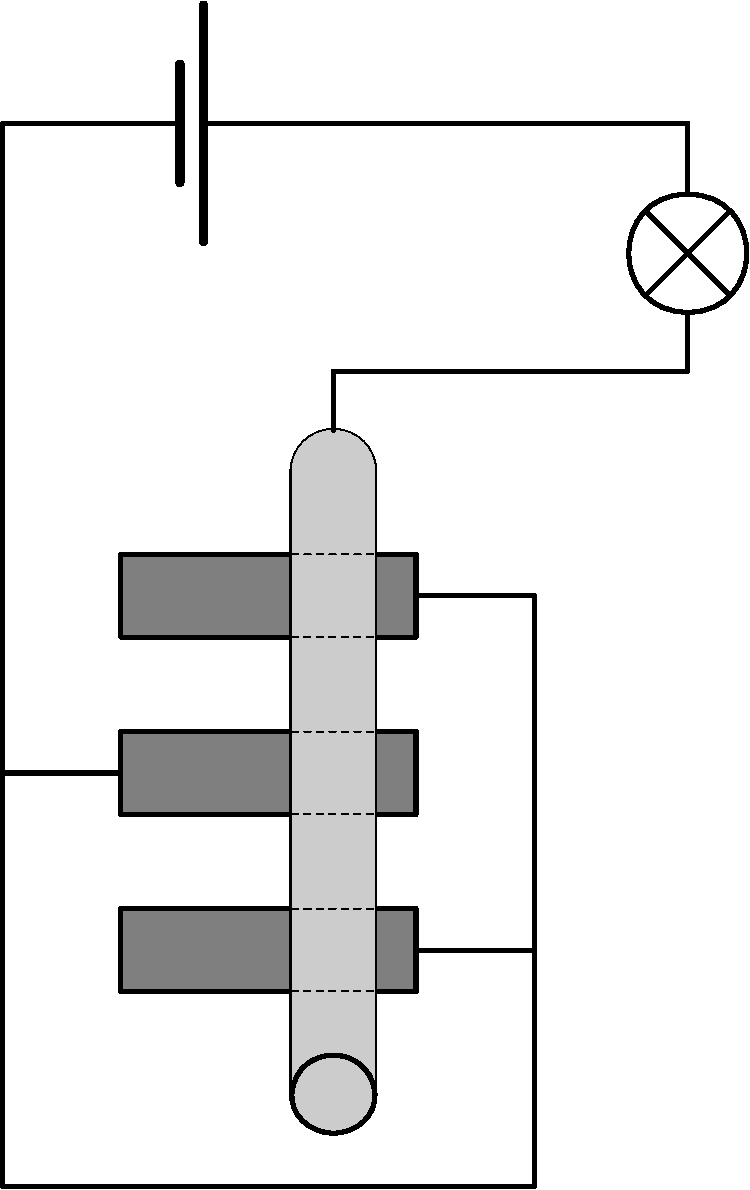
\includegraphics[scale=0.25]{2022-lahg-05-yl.pdf}}
\end{wrapfigure}


Õhukeste grafiitplaatide mõõtmed on 100 $\mu$m $\times$ 1 cm $\times$ 10 cm ning eritakistus on $\rho =  \SI{1}{\Omega m}$. Kolm sellist plaati paiknevad paralleelselt isolaatoril ja igale neist on ühele otstest ühendatud plaadilaiune klemm (ei pea olema tingimata kõigil samas otsas!). Kõik need kolm klemmi on juhtmetega ühendatud patarei ühe otsaga. Patarei teine ots on ühendatud $R = \SI{10}{k \Omega}$ takistust omava tarbija ühe klemmiga. Selle tarbija teine klemm on ühendatud juhtmete kaudu juhist toruga, mis on paigutatud risti üle kõigi kolme paberilipaka nagu näidatud joonisel. Patarei elektromotoorjõud $U =\SI{12}{V}$ ja sisetakistus on tühine.
\\(a) Kui toru puudutab kõiki pabereid $l = \SI{8}{cm}$ nende vasakust otsast, siis rakendub tarbijal ligikaudu võimsus $P = \SI{2,65}{mW}$. Mitu plaati on ühendatud vasakult? 
\\(b) Milline võimsus rakenduks tarbijal, kui liigutada toru nii, et ta puutuks iga paberilipakat vasakust otsast \SI{7}{cm} kauguselt.






\hint

\solu
Grafiigrafiitplaatide käituvad kui reostaadid.
Ristlõikepindala on $100 \cdot 10^{-6} \cdot 1 \cdot 10^{-2} = 10^{-6} \si{m^2}$.
Olgu $l$ toru puutepunkti kaugus vasakust otsast (meetrites).
Vasakult poolt ühendatud plaadi takistus avaldub kujul $R(l)=\rho \frac{l}{S} = 10^6 l $, paremalt poolt ühendatud plaadi takistus avaldub kujul $R(l)= \rho \frac{0.1 - l}{S} = 10^6 (0.1-l) $.
Vasakult poolt ühendatud plaatide arv saab olla 0 kuni 3, vastavate rööbitiühenduses olevate plaatide kui süsteemide kogutakistused avaldub kujul
\[ R_{0v}(l) = \left(\frac{3}{10^6 (0.1-l)} \right)^{-1} =  \frac{10^6}{3} (0.1-l) \]
\[ R_{1v}(l) = \left(\frac{2}{10^6 (0.1-l) } + \frac{1}{10^6 l } \right)^{-1} =  
\left(\frac{2l +(0.1-l)}{10^6 (0.1-l)l }\right)^{-1} = \]
\[ \left(\frac{l +0.1}{10^6 (0.1-l)l }\right)^{-1} =10^6 l\frac{(0.1-l)}{l+0.1} \]
\[ R_{2v}(l) = \left(\frac{1}{10^6 (0.1-l) } + \frac{2}{10^6 l } \right)^{-1} =  
\left(\frac{l +2(0.1-l)}{10^6 (0.1-l)l }\right)^{-1} = \]
\[ \left(\frac{0.2-l}{10^6 (0.1-l)l }\right)^{-1} =10^6 l \frac{(0.1-l)}{0.2-l} \]
\[ R_{3v}(l) = \left(\frac{3}{10^6 l} \right)^{-1} =  \frac{10^6}{3}l\]

Seega võimalikud takistused oleksid
\[R_{0v}(0.08) = \frac{10^6}{3} \cdot (0.1-0.08) = \SI{6667}{\Omega}\]
\[R_{1v}(0.08) = 10^6 \cdot  0.08 \cdot \frac{(0.1-0.08)}{0.08+0.1} = \SI{8889}{\Omega}\]
\[R_{2v}(0.08) = 10^6 \cdot  0.08 \cdot  \frac{(0.1-0.08)}{0.2-0.08} = \SI{13333}{\Omega}\]
\[R_{3v}(0.08) = \frac{10^6}{3} \cdot 0.08 = \SI{26667}{\Omega}\]
Voolutugevused oleksid $I_i=\frac{U}{R_i  + R}$, kus $R = 10^4\si{\Omega}$ ja $U = \SI{12}{\volt}$:
\[ I_{0v}(0.08) = \frac{12}{10^4 + 6667} = 7.2 \cdot 10^{-4} \si{\ampere}\]
\[ I_{1v}(0.08) = \frac{12}{10^4 + 8889} = 6.353 \cdot 10^{-4} \si{\ampere}\]
\[ I_{2v}(0.08) = \frac{12}{10^4 + 13333} = 5.143 \cdot 10^{-4} \si{\ampere}\]
\[ I_{3v}(0.08) = \frac{12}{10^4 + 26667} = 3.273 \cdot 10^{-4} \si{\ampere}\]
Vastavad võimsused $P_i = (I_i)^2 \cdot R$ oleksid siis
\[ P_{0v}(0.08) = (7.2 \cdot 10^{-4})^2 \cdot 10^4 = 5.184 \cdot 10^{-3}  \si{\watt}\]
\[ P_{1v}(0.08) = (6.353 \cdot 10^{-4})^2 \cdot 10^4 = 4.036 \cdot 10^{-3}  \si{\watt}\]
\[ P_{2v}(0.08) = (5.143 \cdot 10^{-4})^2 \cdot 10^4 = 2.645 \cdot 10^{-3}  \si{\watt}\]
\[ P_{3v}(0.08) = (3.273 \cdot 10^{-4})^2 \cdot 10^4 = 1.071 \cdot 10^{-3}  \si{\watt}\]
Seega kehtib meil olukord, kus kaks plaati on ühendatud vasakult ja üks paremalt.

Pärast toru liigutamist muutub $l=\SI{0.07}{\meter} $.
Arvutab uue takistuse
\[ R_{2v}(0.07) =  10^6 \cdot 0.07 \cdot  \frac{(0.1-0.07)}{0.2-0.07} = \SI{16154}{\Omega} \]
Arvutab uue voolutugevuse
\[ I_{2v}(0.07) = \frac{12}{10^4 + 16154} = 4.588 \cdot 10^{-4} \si{\ampere}\]
Arvutab  uue võimsuse
\[ P_{2v}(0.07) = (4.588 \cdot 10^{-4})^2 \cdot 10^4 = 2.105 \cdot 10^{-3}  \si{\watt}\]
\probend